\chapter{Application Layer}




\section{Principles of the Network Applications}

\subsection{Network Applicatoin Architectures}

\hf\textbfit{Application Architecture} is designed by the application developer and \textit{dictates how the application is structured} over
various end systems.\\

Two predominant architectural paradigms:
\begin{enumerate}
    \item client-server architecture
    \item peer-to-peer(P2P) architecture
\end{enumerate}

\subsubsection{Client-Server}

\begin{enumerate}
    \item Server: the always-on host which services requests from many other hosts.
    \item Client: the end host whic request services from the server.
\end{enumerate}

Note that with the client-server architecture, clients do not directly communicate with each
other;for example, in the Web application, two browsers do not directly communi-
cate.\\
Another characteristic of the client-server architecture is that \textbfit{the server has a
    fixed, well-known address, called an IP address}. Because
the server has a fixed, well-known address, and because the server is always on, a
client can always contact the server by sending a packet to the server’s IP address.\\
Some well-known applications within client-server architecture:
\begin{enumerate}
    \item Web
    \item FTP
    \item Telnet
    \item e-mail
\end{enumerate}



\subsection{P2P architecture}

There is minimal (or no) reliance on dedicated servers in
data centers.Instead the application exploits direct communication between pairs of
intermittently connected hosts, called peers.\\

Characteristics that P2P architecture has:
\begin{enumerate}
    \item \textbfit{Self-Scalability}:although each peer generates
          workload by requesting files, each peer also adds service capacity to the system
          by distributing files to other peers.
    \item Cost effictive: normally don’t require significant server infrastructure and server bandwidth
\end{enumerate}

The problems that P2P need to face:
\begin{enumerate}
    \item ISP's asymmetrical bandwidth usage: ISPs are dimensioned for much more downstream than upstream traffic. But in p2p architecture, every residential ISPs will face a gigantic amount of upstream traffic.
    \item Security: Because of their highly distributed and open nature, P2P applications can be a challenge to secure.
    \item Incentives: Need users to volunteer bandwidth, storage, and computation resources to application.
\end{enumerate}

\subsection{Transport services available to applications}

\hf We can broadly classify the possible services along four dimensions:
\begin{enumerate}
    \item Reliable data transfer
    \item Throughput
    \item Timing
    \item Security
\end{enumerate}


\newpage

\section{Socket}

\hf
Most applications consist of pairs of communicating processes, with the two processes in each pair sending messages to each other.\\
\textbfit{Socket}: the interface that a process sends messages into, and receives messages from.

\begin{figure}[!h]
    \centering
    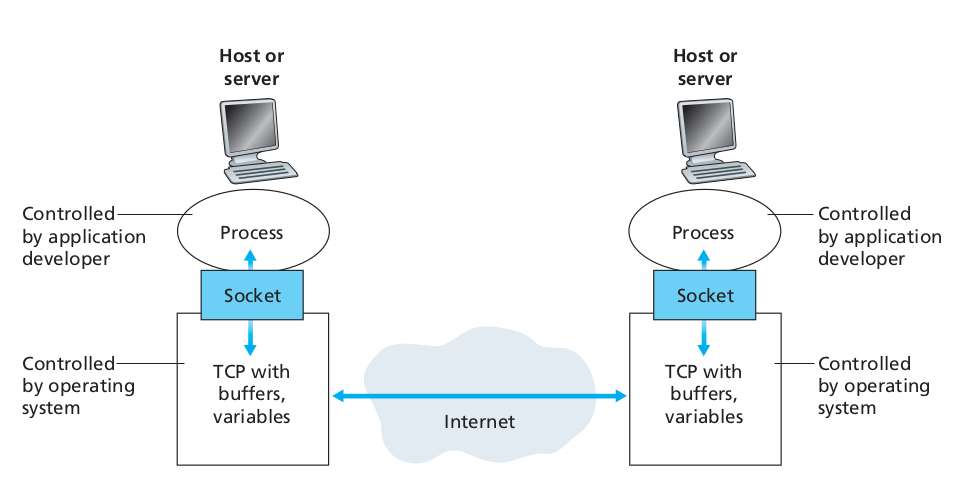
\includegraphics[width=0.7\textwidth]{chapters/chapter2/socket.png}
    \caption{Socket}
    \label{c2_socket}
\end{figure}

Socket is also referred as the API between the application and the network. The developer has control
of everything on the application-layer side but only little control of the transport-layer side of the socket:
\begin{enumerate}
    \item the choice of transport protocol
    \item fix a few transport-layer parameters such as maximum buffer and maximum segment sizes.
\end{enumerate}

\subsection{Address Processes}

\hf
Similarly, in order for a process running on one host to send packets to a
process running on another host, the receiving process needs to have an address.
In particular:
\begin{enumerate}
    \item The address of the host:\ \textbfit{IP address}.
    \item an identifier that specifies the receiving process in the destination host: \textbfit{Port number}.
\end{enumerate}

Some ports are reserved by well-known applications. For example, a Web server has port number 80. A mail server process has port number 25.


\newpage
\section{The Web and HTTP}

\hf
The Web operates on demand.
\subsection{Overiew of HTTP}

The Web's application-layer protocol: HTTP(HyperText Transfer Protocol). HTTP is implemented both in client program and server program.
HTTP defines the structure of the messages and how the client and server exchange the messages.\\
\begin{center}
    Web browsers: Client side of HTTP.\\
    Web servers: Server side of HTTP, addressable by a URL.
\end{center}


\subsubsection{HTTP uses TCP}

\hf
The flow:
\begin{enumerate}
    \item The HTTP client initiates a TCP connection with the server.
    \item The HTTP client sends request messages into its socketnd and waits to receive HTTP response messages from its socket interface.
    \item The HTTP server receives request from its socket and sends response into its socket interface.
    \item The HTTP client receives the response.
\end{enumerate}

Another important thing is that HTTP is \tbi{stateless protocol}.


\subsection{HTTP with different connections}

\hf
There are two connection types for HTTP:
\begin{enumerate}
    \item Non-persistent connection: the application sends response using existing TCP connection.
    \item Persistent connection: the appication sends each response with a new TCP connection.
\end{enumerate}

\tbi{RTT(Round Trip Time)}

Non-persistent connection will take around two RTT for a single HTML file,and for each TCP established the TCP
variables need to be stored in both client and server side. This can place a significant burden on the Web server.\\

Persistent connection will only take one RTT once the connection is
established, and persistent connection with pipelining is the default mode of the HTTP.


\subsection{HTTP Request Format}

\hf
\begin{center}
    GET /somedir/page.html HTTP/1.1\\
    Host: www.someschool.edu\\
    Connection: close\\
    User-agent: Mozilla/5.0\\
    Accept-language: fr
    \label{c2_http_request}
\end{center}

The first line is called: the \tbi{request line};
The subsequent lines are called: the \tbi{header lines}.\\
The request line has three fields:
\begin{enumerate}
    \item The method field: including \tbi{GET,POST,HEAD,PUT} and \tbi{DELETE}.
    \item The URL field
    \item The HTTP version field
\end{enumerate}

The great majority of HTTP request messages use the GET method. The GET
method is used when the browser requests an object, with the requested object iden tified in the URL field.\\

The header line \tbi{Host: wwwwww.someschool.edu} specifies the host on which the object resides. The header line \tbi{Connection: close}
tells the server close the connection after sending the requested object. The \tbi{User-agent} and \tbi{Accept-Language} are self-explanatory.\\

\newpage

\begin{figure}[!h]
    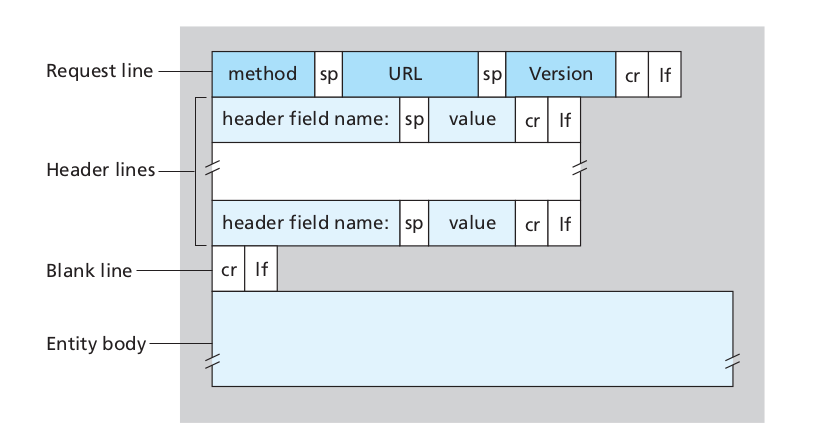
\includegraphics[width=0.95\textwidth]{chapters/chapter2/HTTP_Format.png}
    \caption{General format of an HTTP request message}
    \label{c2_http_format}
\end{figure}

The \tbi{entity body} is empty with \tbi{GET} method, but is used in \tbi{POST} method:HTTP client
often uses the POST method when the user fills out a form. For example, when a
user provides search words to a search engine. \\
However HTML forms often use the \tbi{GET} method and include the inputted data in the request URL. For example, inputted data is banana and money,
then the URL will look like \underlineit{www.somesite.com/search?monkeys\&bananas}.
The \tbi{HEAD} method only responds with an HTTP message but it leaves out the requested object(used to debug).\\
The \tbi{PUT} method allows a user to upload an object to specific path on specific Web server. It is also used by applications that need to
upload objects to Web servers.\\
The \tbi{DELETE} method allows a user, or an application, to delete an
object on a Web server.


\subsection{HTTP Reponse Format}




\begin{center}
    HTTP/1.1 200 OK\\
    Connection: close\\
    Date: Tue, 09 Aug 2011 15:44:04 GMT\\
    Server: Apache/2.2.3 (CentOS)\\
    Last-Modified: Tue, 09 Aug 2011 15:11:03 GMT\\
    Content-Length: 6821\\
    Content-Type: text/html\\
    (data data data data data ...)
\end{center}

The example has three sections: an initial \tbi{status line}, six \tbi{header line}, and then the \tbi{entity body}.\\
\subsubsection{The status line has three fields:}

\begin{enumerate}
    \item The protocol version field
    \item A status code: 200 in the example
    \item A corresponding status message.
\end{enumerate}

\subsubsection{The six header lines:}

\begin{enumerate}
    \item \tbi{Connection: close} header line: tell the client that it is going to close the TCP connection.
    \item The \tbi{Date:} header line indicates the time and date when the HTTP response was created and sent by the server.
    \item The \tbi{Server:} header line indicates that the message was generated by an Apache Web server.
    \item The \tbi{Last-Modified:} header line indicates the time and date when the object was created or last modified.
    \item The \tbi{Content-Length:} header line indicates the number of bytes in the object being sent.
    \item The \tbi{Content-Type:} header line indicates that the object in the entity body is HTML text.
\end{enumerate}


\subsubsection{General format of an HTTP response message}

\begin{figure}[!h]
    \centering
    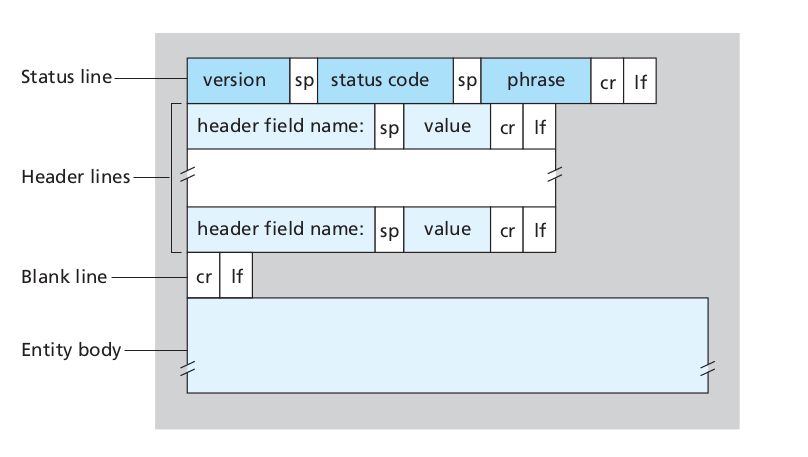
\includegraphics[width=0.9\textwidth]{chapters/chapter2/HTTP_Reponse_Message.png}
    \caption{General format of an HTTP response message}
    \label{c2_http_response}
\end{figure}

Some common status codes and associated phrases include:
\begin{enumerate}
    \item \tbi{200 OK}: Request succeeded and the information is returned in the response.
    \item \tbi{301 Moved Permanently}: Requested object has been permanently moved;
          the new URL is specified in Location: header of the response message. The
          client software will automatically retrieve the new URL.
    \item \tbi{400 Bad Request}: This is a generic error code indicating that the request
          could not be understood by the server.
    \item \tbi{404 Not Found}: The requested document does not exist on this server.
    \item \tbi{505 HTTP Version Not Supported}: The requested HTTP protocol
          version is not supported by the server.
\end{enumerate}


\subsection{Cookies}

\hf
HTTP use cookies to identify users.

\begin{figure}[!h]
    \centering
    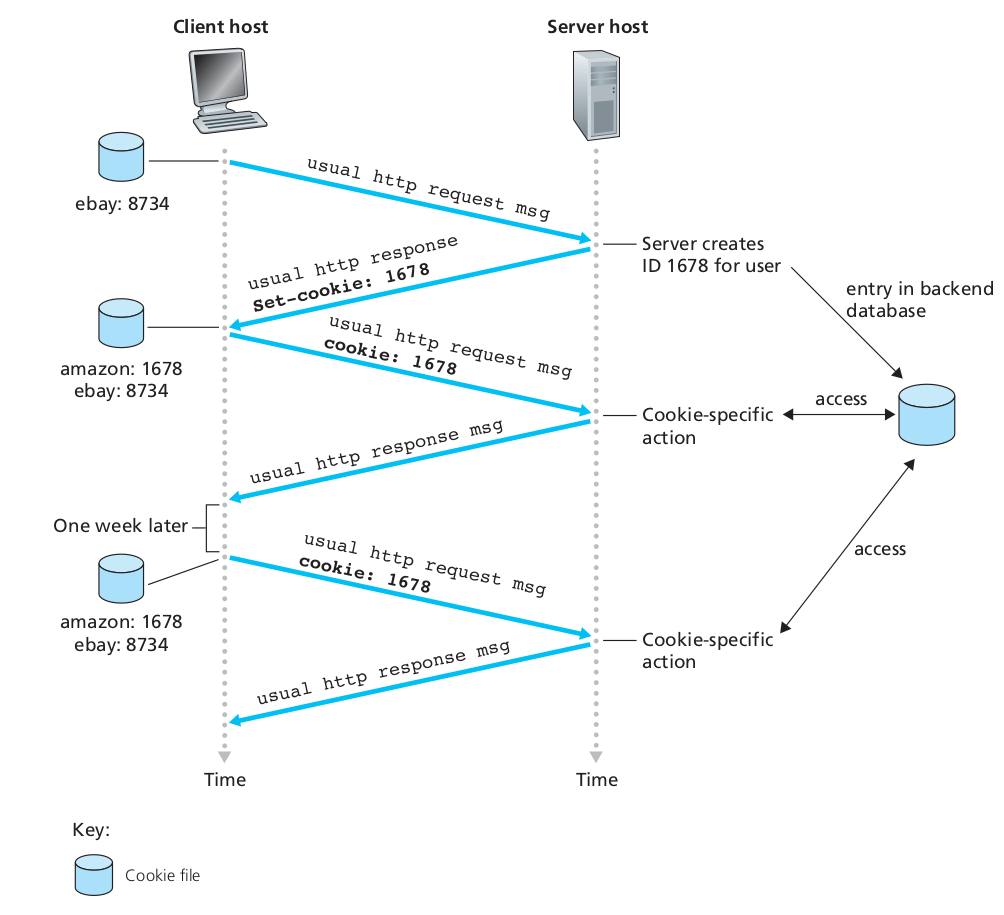
\includegraphics[width=0.9\textwidth]{chapters/chapter2/UserState_cookie.png}
    \caption{Use cookie to identify users}
    \label{c2_cookies}
\end{figure}

\subsubsection{Major cookies components}
\begin{enumerate}
    \item A cookie header line in the HTTP response message.
    \item A cookie header line in the HTTP request message.
    \item A cookie file kept on the user’s end system and managed by the
          user’s browser.
    \item A back-end database at the Web site.
\end{enumerate}

Flows of using cookies:
\begin{enumerate}
    \item Alice send HTTP request message without a cookie header line.
    \item The server generates a new cookies number and stores it to the database.Then repsonses with Set-cookie: header \tbi{Set-cookie: 1678}.
    \item When Alice receives the response message, her browsers appends a line to the special cookie file that it manages.
    \item In the following requests, Alice's browser will include the cookie for the server in the header lines. Like \tbi{Cookie: 1678}.
    \item The server will identify Alice with the cookie it receives in the header liens.
\end{enumerate}



\subsection{Web Caching}
A \tbi{Web cache}—also called a \tbi{proxy server}—is a network entity that satisfies HTTP
requests on the behalf of an origin Web server. \underlineit{The Web cache is both a client and a server}.

\begin{figure}
    \centering
    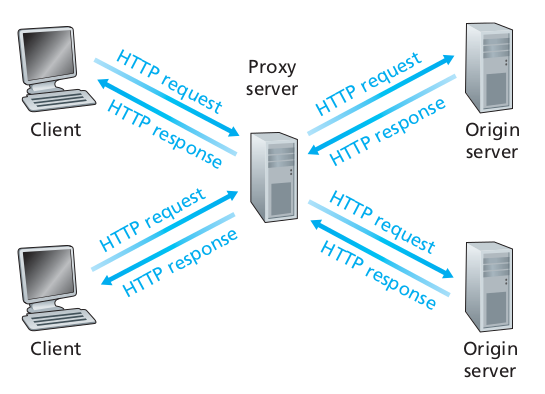
\includegraphics[width=0.6\textwidth]{chapters/chapter2/web_cache.png}
    \caption{Web Caching}
    \label{c2_web_caching}
\end{figure}

The web caching process:
\begin{enumerate}
    \item The browser establishes TCP connection to the Web cache and sends HTTP request for the object to the Web cache
    \item The Web cache checks to see if it has a copy of the object stored locally. If it
          does, the Web cache returns the object within an HTTP response message to
          the client browser.
    \item If the Web cache does not have a copy of the object, it sends HTTP request for the object to the origin server.
    \item The web cache receives the object from the origin server with HTTP response, it stores a copy of the object and sends back to the browser.
\end{enumerate}

Typically a Web cache is purchased and installed by an ISP. For example, a uni-
versity might install a cache on its campus network and configure all of the campus
browsers to point to the cache.Or a major residential ISP (such as AOL) might
install one or more caches in its network and preconfigure its shipped browsers to
point to the installed caches.\\

\subsubsection{Advantage of using a web cache/proxy server}

\begin{enumerate}
    \item A Web
          cache can substantially reduce the response time for a client request, particularly if the
          bottleneck bandwidth between the client and the origin server is much less than the bot-
          tleneck bandwidth between the client and the cache.
    \item Web caches can substantially reduce traffic on an institution’s access link to the Internet. By reducing traffic, the institution does not have to upgrade bandwidth as quickly, thereby
          reducing costs.
    \item Web caches can substantially reduce Web traffic in the Internet as a whole, thereby improving performance for all applications.
\end{enumerate}


\insertImage{width=0.4\textwidth}{chapters/chapter2/Cache_example.png}{Adding a cache to the institutional network}{c2_cache_example}

Suppose that the average object size is 1Mbits and that the average request rate from instution's
browsers to origin server is 15 requests per second.\\
The traffic intensity on the LAN is:
\begin{equation}
    (15 requests/sec) \cdot (1 Mbits/request) / (100Mps) = 0.15
    \label{c2_lan_traffic_intensity}
\end{equation}

The traffic intensity on the access link(from the Internet router to institution
router) is:
\begin{equation}
    (15 requests/sec) \cdot (1 Mbits/request) / (15Mps) = 1
    \label{c2_accessLink_traffic_intensity}
\end{equation}
Which is really bad and goes to infinite.

However, when we use the Web cache in the \autoref{c2_cache_example} when the hit rate is 0.4,
we will a traffic intensity on the access link:
\begin{equation}
    (15*0.6 requests/sec) \cdot (1 Mbits/request) / (15Mps) =0.6
\end{equation}
Which is much better.

\subsubsection{The conditional \textbf{GET}}

\hf
The Web cache uses \tbi{conditional GET} to check whether the copy of the object is up to date.
A HTTP request message is \tbi{conditional GET} if
\begin{enumerate}
    \item The request message uses the \tbi{GET} method.
    \item The request message includes an \tbi{If-Modified-Since:} header line.
\end{enumerate}

First, on the behalf of a requesting browser, a proxy cache sends a request message
to a Web server:

\begin{center}
    GET /fruit/banana HTTP/1.1\\
    HOST: www.walmart.ca
\end{center}

Second, the Web server receives the HTTP response from origin server:

\begin{center}
    HTTP/1.1 200 OK\\
    Date: Sat, 8 Oct 2011 15:39:32\\
    Server: Apache/1.3.0 (UNIX)\\
    Last-Modified: Wed, 7 Sep 2011 09:23:24\\
    Content-Type: image/gif\\
    (data data data data data ...)
\end{center}

The Web cache would forward the object to the requesting browser and store a copy of it.
When the next time someone sends a same request message, the Web cache would send a \tbi{conditional
    GET}:

\begin{center}
    GET /fruit/banana HTTP/1.1\\
    HOST: www.walmart.ca\\
    If-modified-since: Wed, 7 Sep 2011 09:23:24
\end{center}

Suppose the object is not updated after the last \tbi{GET}, the origin server would response:

\begin{center}
    HTTP/1.1 304 Not Modified\\
    Date: Sat, 15 Oct 2011 15:39:29\\
    Server: Apache/1.3.0 (Unix)\\
    (empty entity body)
\end{center}

\tbi{304 Not Modified} indicates that the requested object is not modified since Wed, 7 Sep 2011 09:23:24.
Therefore, it doesn't attach the data in the entity. The Web cache would forward the local copy of the
object back to the browser.\\

Note that an HTTP request/response message is negligible. Therefore, a \tbi{conditional GET} does
not cause delay to forward the copy of the object to the browser if there is no modification made.



\newpage
\section{FTP: File Transfer Protocol}

\insertImage{width=0.8\textwidth}{chapters/chapter2/FTP.png}{FTP}{c2_FTP}

\subsection{Overview of FTP}

\hf
In \autoref{c2_FTP}:
\begin{enumerate}
    \item User interacts with FTP with an FTP user agent and provides the hostname of the remote host.
    \item The process in the local host starts a TCP connection with the FTP server process.
    \item The user provides identification and password via the established TCP connection.
    \item The server authenticates and authorizes the user.
    \item User can copy files from(into) the server(local).
\end{enumerate}


\subsection{Control connection and data connection}

\hf
The \tbi{FTP} uses \tbi{two parallel TCP connections} to transfer a file, a
\tbi{control connection} and a \tbi{data connection}.\\

The \tbi{control connection} is used for sending control information between processes -
information such as user identification, password, commands to change remote directory,
and commands to "put" and "get" files.\\

The \tbi{data connection} is used to actually send a file.\\
Because TCP uses a seperate control connection, FTP authenticateis said to send its control information
\tbi{out-of-band}. HTTP sends request and response header lines into the same TCP connection that
carries the transferred file itself. Therefore, HTTP is said to send its control information \tbi{in-band}.

\insertImage{width = 0.6\textwidth}{chapters/chapter2/FTP_control_and_data.png}{Control and data connections}{c2_ftp_control_data}

\begin{enumerate}
    \item The client process starts an FTP session with a remote host.
    \item The client process initiate a control TCP connection with the server process on \tbi{port 21}.
    \item The client process sends user identification and password over the control connection.
    \item The client process sends a command via control connection.
    \item The server process receives a command for a file transfer over the control connection.
    \item The server initiates a TCP data connection to client process on \tbi{port 20}.
\end{enumerate}



\utbi{Note that FTP sends exactly one file over the data connection and closes the data connection.}
\utbi{If, during the same session, the user wants to transfer another file,
    FTP opens another data connection.}
\utbi{Thus, with FTP, the control connection remains open throughout the duration of the user session}.
\utbi{New data connection is created for each file transferred within a session.}

\begin{center}
    \begin{enumerate}
        \item Data connection is non-persistent.
        \item Control connection is persistent.
    \end{enumerate}
\end{center}


Also, the FTP server must maintain \tbi{state} about the user:
\begin{enumerate}
    \item Associate the control connection with specific user account
    \item Keep track of the user's current directory in the remote diretory tree.
\end{enumerate}

Keeping track of this state information for each
ongoing user session significantly constrains the total number of sessions that FTP
can maintain simultaneously.

\subsection{FTP commands and replies}


\hf
The commands, from client to server, and replies, from server to
client, are sent across the control connection in 7-bit ASCII format. FTP commands
are readable by people. Each command consists of four uppercase ASCII characters, some with optional arguments.\\

Some common commands:
\begin{enumerate}
    \item USER username: Used to send the user identification to the server.
    \item PASS password: Used to send the user password to the server.
    \item LIST: Used to ask the server to send back a list of all the files in the current
          remote directory. The list of files is sent over a (new and non-persistent) data
          connection.
    \item RETR filename: Used to retrieve (that is, get) a file from the current direc-
          tory of the remote host. This command causes the remote host to initiate a data
          connection and to send the requested file over the data connection.
    \item STOR filename: Used to store (that is, put) a file into the current directory
          of the remote host.
\end{enumerate}

Each command is followed by a reply, sent from server to client.\\

Some common replies:
\begin{enumerate}
    \item 331 Username OK, password required
    \item 125 Data connection already open; transfer starting
    \item 425 Can't open data connection
    \item Error writing file
\end{enumerate}


\newpage

\section{Electronic Mail in the Internet}

\hf
\insertImage{width=0.8\textwidth}{chapters/chapter2/email_system}{High-level view of email system}{c2_email}

Three major components of in \autoref{c2_email}:
\begin{enumerate}
    \item User agents
    \item Mail servers
    \item SMTP: Simple Mail Transfer Protocol
\end{enumerate}

Sender's view:
\begin{enumerate}
    \item User agent allows the sender to compose the message.
    \item The user agent sends the message to the email server.
    \item The message is placed in the mail server's outgoing message queue.
    \item The recipent retrieves the message from his/her mailbox in the mail server.
\end{enumerate}

Mail servers form the core of the e-mail infrastructure. Each recipent has
a \tbi{maibox} located in one of the mail servers. The mailbox manages and maintains
the messages that have been sent to the recipent.\\

The typical message's journey:
\begin{enumerate}
    \item Sender's user agent.
    \item Sender's mail server.
    \item Recipent's mail server.
    \item Recipent's mailbox.
\end{enumerate}

The sender mail server must also deal with failures in the recipent mail
box: If the sender server can not delivery mail to the recipent server,
sender server holds the message in a message
queue and attempts to transfer the message later.


\subsection{SMTP: Simple Mail Tranfer Protocol}

\hf
SMTP uses TCP to transfer mail \tbi{from the sender's mail server to the
    recipent's mail server}.\\

When a mail server sends mail to other mail servers, it acts as an SMTP
client. When a mail server receives mail from other mail servers, it acts as
an SMTP server.\\

SMTP restricts the body of all mail messages to simple 7-bit ASCII.

\insertImage{width=0.8\textwidth}{chapters/chapter2/alice_and_bob.png}{Alice sends a message to Bob}{c2_alice_bob_smtp}

When Alice sends Bob an ASCII message:
\begin{enumerate}
    \item Alice invokes her user agent for e-mail, provides Bob’s e-mail address (for
          example, bob@someschool.edu), composes a message, and instructs the
          user agent to send the message.
    \item Alice’s user agent sends the message to her mail server, where it is placed in a
          message queue.
    \item The client side of SMTP, running on Alice’s mail server, sees the message in
          the message queue. It opens a TCP connection to an SMTP server, running on
          Bob’s mail server.
    \item After some initial SMTP handshaking, the SMTP client sends Alice’s message
          into the TCP connection.
    \item At Bob’s mail server, the server side of SMTP receives the message. Bob’s
          mail server then places the message in Bob’s mailbox.
    \item Bob invokes his user agent to read the message at his convenience.
\end{enumerate}

\subsubsection{Detailed SMTP}

\hf
SMTP does not use intermediate email servers for sending email. SMTP establishes a connection
to port 25 at the server SMTP. Once the connection is established, the server and
client perform some application layer-handshaking. SMTP client indicates the e-mail
address of the sender and the e-mail address of the recipent. Once the handshaking is
complete, the client sends the message and repeats if there are more messages to send
to the same server.\\

Example:
\begin{enumerate}
    \item S: 220 hamburger.edu
    \item C: HELO crepes.fr
    \item S: 250 Hello crepes.fr, pleased to meet you
    \item C: MAIL FROM: <alice@crepes.fr>
    \item S: 250 alice@crepes.fr ... Sender ok
    \item C: RCPT TO: <bob@hamburger.edu>
    \item S: 250 bob@hamburger.edu ... Recipient ok
    \item C: DATA
    \item S: 354 Enter mail, end with “.” on a line by itself
    \item C: Do you like ketchup?
    \item C: How about pickles?
    \item C: .
    \item S: 250 Message accepted for delivery
    \item C: QUIT
    \item S: 221 hamburger.edu closing connection
\end{enumerate}

\subsubsection{Comparison with HTTP}

\hf Common: Both persistent HTTP and SMTP use persistent connections. \\

Difference:
\begin{enumerate}
    \item The HTTP is maily a\tbi{pull protocol}; SMTP is primarily a \tbi{push protocol}.
    \item The message has to be encoded into 7-bit ASCII while using SMTP; HTTP doesn't impose this restriction.
    \item HTTP encapsulates each object in its own HTTP response message; Internet mail places all of the message's objects into one message.
\end{enumerate}


\subsubsection{Mail message format}

\hf
A typical message header looks like this:
\begin{center}
    From: alice@crepes.fr\\
    To: bob@hamburger.edu\\
    Subject: Searching for the meaning of life.
\end{center}

\subsubsection{Mail access protocol}

\hf
Recall that a mail server manages mailboxes and runs the
client and server sides of SMTP. If Bob's mail server were to reside
on his local PC, then Bob's PC would have to remain always on, and connected
to the Internet. Instead, a typical user runs a user agent on the local PC but accesses
its mailbox stored on an always-on shared mail server.This mail server is shared
with other users and is typically maintained by the user’s ISP.\\

How can Bob retrieve his email from the mailbox?
\insertImage{width=0.8\textwidth}{chapters/chapter2/Retrieve_email.png}{Retrieve mail from mailbox}{c2_retrieve_from_mailbox}

Protocols like :\tbi{POP3} (Post Office Protocol version 3.0), \tbi{IMAP} (Internet Mail
Access Protocol), and \tbi{HTTP} are used to pull mail from mail server to the recipent's
agent.

\subsubsection{POP3}

\hf POP3 is extremly simple mail access protocol, and it is short and readable. Because the protocol is so simple, its functionality is
rather limited.\\

POP3 begins when the user agent opens a TCP connection to mail server on \tbi{port 110}.With the TCP connection estab-
lished, POP3 progresses through three phases: authorization, transaction, and update.\\

During the first phase, authorization, the user agent sends a username and a password
(in the clear) to authenticate the user.\\


During the second phase, transaction, the user
agent retrieves messages; also during this phase, the user agent can mark messages
for deletion, remove deletion marks, and obtain mail statistics.\\

The third phase,
update, occurs after the client has issued the quit command, ending the POP3
session; at this time, the mail server deletes the messages that were marked for
deletion.\\

In a POP3 transaction, the user agent issues commands, and the server responds
to each command with a reply. There are two possible responses: \tbi{+OK} (sometimes
followed by server-to-client data), used by the server to indicate that the previous
command was fine; and \tbi{-ERR}, used by the server to indicate that something was
wrong with the previous command.\\

The sequence of commands issued by a POP3 user agent depends on which
of these two modes the user agent is operating in. In the download-and-delete mode,
the user agent will issue the list, retr, and dele commands.\\

Transaction phrase example:
\begin{enumerate}
    \item C: list
    \item S: 1 498
    \item S: 2 912
    \item S: .
    \item C: retr 1
    \item S: (blah blah \dots
    \item S: \dots \dots \dots
    \item S: \dots \dots \dots blah)
    \item S: .
    \item C: dele 1
    \item C: retr 2
    \item S: (blah blah \dots
    \item S: \dots \dots \dots
    \item S: \dots \dots \dots blah)
    \item S: .
    \item C: dele 2
    \item C: quit
    \item S: +OK POP3 server signing off
\end{enumerate}

\subsection{IMAP: Internet Mail Access Protocol}

\hf
The POP3 doesn't provide any means of a user to create remote folders and assign
messages to folders. => IMAP is introduced to solve this problem, but it is significantly
more complex.\\

An IMAP server will associate each message with a folder; when a message first
arrives at the server, it is associated with the recipient’s INBOX folder. The recipient
can then move the message into a new, user-created folder, read the message, delete
the message, and so on.\\

Another important feature of IMAP is that it has commands that permit a user
agent to obtain components of messages. For example, a user agent can obtain just
the message header of a message or just one part of a multipart MIME message.
This feature is useful when there is a low-bandwidth connection between the user agent and its mail server.


\subsection{Web-Based E-mail}

\hf
Hotmail introduced Web-based access in the mid 1990s.With this service, the user agent is an ordinary Web browser,
and the user communicates with its remote mailbox via HTTP.


\newpage
\section{DNS: Domain Name System — The Internet's Directory service}

Domain name vs Host name: hostname.domain.com
\begin{enumerate}
    \item Hostname is the name given to the end-point(a machine).
    \item Domain is the name given to the "network".
\end{enumerate}

\hf
Internet hosts can be identified by different ways: by \tbi{Hostname}, such as
www.google.com or so-called \tbi{IP address}.


\subsection{Services Provided by DNS}

\hf
From my perspective, DNS does one thing: search up IP address by hostname.\\
Note that \tbi{DNS uses UDP and uses port 53}.

The DNS is
\begin{enumerate}
    \item a distributed database implemented in a hierarchy of \tbi{DNS servers}.
    \item an application-layer protocol that allows host to query the distributed database.
\end{enumerate}

DNS is commonly employed by other application-layer protocols---including HTTP,
SMTP, and FTP --- to translate user-supplied hostnames to IP addresses. In order for
the user's host to be able to send an HTTP request message to the Web server www.someschool.edu, the user’s host must first obtain
the IP address of www.someschool.edu. This is done as follows.

\begin{enumerate}
    \item The same user machine runs the client side of the DNS application.
    \item The browser extracts the hostname, www.someschool.edu, from the URL
          and passes the hostname to the client side of the DNS application
    \item The DNS client sends a query containing the hostname to a DNS server.
    \item The DNS client eventually receives a reply, which includes the IP address for
          the hostname.
    \item Once the browser receives the IP address from DNS, it can initiate a TCP con-
          nection to the HTTP server process located at port 80 at that IP address.
\end{enumerate}


DNS adds an additional delay (sometimes substantial) - to the Internet applications
that use it. Fortunately, the
desired IP address is often cached in a “nearby” DNS server, which helps to reduce
DNS network traffic as well as the average DNS delay.


\tbi{DNS provides a few other important services:}

\begin{enumerate}
    \item Host aliasing
    \item Mail server aliasing
    \item Load distribution: DNS is also used to perform load distribution among replicated servers, such as replicated Web servers. When the client makes a DNS query for a name
    mapped to a set of addresses, the server responds with the entire set of IP addresses,
    but rotates the ordering of the addresses within each reply.
\end{enumerate}


\subsection{Overview of How DNS Works}

In order to deal with the issue of scale, the DNS uses a large number of servers,
organized in a hierarchy fashion and distributed around the world. No single DNS
server has all the mappings for all of the hosts in the Internet. Instead, the mappings
are distributed across the DNS servers.\\

\insertImage{width=0.7\textwidth}{chapters/chapter2/DNS_hierarchy.png}{DNS Hierarchy}{c2_dns_hierarchy}

There are three classes of DNS servers — root DNS servers, top-level domain (TLD) DNS
servers, and authoritative DNS servers — organized in a hierarchy in \autoref{c2_dns_hierarchy}.\\

When searching for www.amazon.com:
\begin{enumerate}
    \item The client contacts one of the root servers.
    \item The root server returns IP addresses for TLD servers for top-level domain com.
    \item The client contacts one of the TLD servers.
    \item The TLD server returns  IP addresses of authoritative servers for amazon.com.
    \item The client contacts one of the authoritative servers for amazon.com.
    \item The authoritative server returns the IP for www.amazon.com
\end{enumerate}


Root DNS servers: There are 13 root DNS servers in 2012:
\insertImage{width=0.7\textwidth}{chapters/chapter2/DNS_root_servers.png}{DNS Root Servers in 2012}{c2_dns_root_servers}

Top-level domain(TLD) servers:\\
These servers are responsible of top-level domains suck as com, org, net,
edu, and gov.\\
\newline
Authoritative DNS servers:\\
Every organization with publicly accessible hosts on the Internet must provide
publicly accessible DNS records that map the names of those hosts to IP addresses.
\newline
Local DNS servers:\\
A local DNS does not strictly belong to the hierarchy of servers but it is nevertheless
central to the DNS architecture. When a host makes a DNS query, the query is
sent to the local DNS server, which acts a proxy, forwarding the query into the DNS
server hierarchy.


\insertImage{width=0.6\textwidth}{chapters/chapter2/Interaction_of_various_DNS_servers.png}{Interaction of the various DNS servers}{c2_dns_servers_interaction}

Local DNS server services as a cache.The idea behind DNS caching is very simple. In a query chain, when a
DNS server receives a DNS reply (containing, for example, a mapping from a host-
name to an IP address), it can cache the mapping in its local memory.\\
\newline

The example in \autoref{c2_c2_dns_servers_interaction} makes use of both \tbi{recursive queries} and 
\tbi{iterative} queries. The query sent from cis.poly.edu to dns.poly.edu is a
recursive query, since the query asks dns.poly.edu to obtain the mapping on its behalf. But the subsequent three queries are iterative since all of the replies are
directly returned to dns.poly.edu. In theory, any DNS query can be iterative or
recursive.


\insertImage{width=0.8\textwidth}{chapters/chapter2/Recursive_queries.png}{Recursive Queries}{c2_recursive_queries}

In the \autoref{c2_recursive_queries} makes use of \tbi{recursive queries}.

\subsection{DNS records and messages}

The DNS servers that together implement the DNS distributed database store
resource records (RRs), including RRs that provide hostname-to-IP address map-
pings.\\

A resource record is a four-tuple that contains the following fields:
\begin{center}
    (Name, Value, Type, TTL)
\end{center}

\tbi{TTL} is the time to live of the resource record; it determines when
a resource should be removed from a cache.

\tbi{Type} field:
\begin{enumerate}
    \item If Type = A, then Name is a hostname and Value is the IP address for the hostname.Example,(relay1.bar.foo.com, 145.37.93.126, A, TTL holder).
    \item If Type = NS, then Name is a domain and Value is the hostname of an authoritative DNS server that knows how to obtain the IP addresses for hosts in the domain. Example,(foo.com, dns.foo.com, NS, TTL).
    \item If Type = CNAME, then Name is an alias hostname and Value is the canonical name for the hostname. Example(foo.com, relay1.bar.foo.com, CNAME, TTL).
    \item If Type = MX, then Name is an alias hostname of a mail server and the Value is the canonical name of the mail server. Example(foo.com, mail.bar.foo.com, MX, TTL).
\end{enumerate}

\subsection{DNS messages}

\insertImage{width=0.7\textwidth}{chapters/chapter2/DNS_message_format.png}{DNS message format}{c2_dns_format}
\hf There only two kinds of DNS messages: Query and Reply. Furthermore, both
query and reply messages have the same format, as shown in \autoref{c2_dns_format}.\\
\begin{enumerate}
    \item The first 12 bytes is the header section, which has a number of fields. The first field
    is a 16-bit number that identifies the query. This identifier is copied into the reply
    message to a query, allowing the client to match received replies with sent queries.
    There are a number of flags in the flag field. A 1-bit query/reply flag indicates
    whether the message is a query (0) or a reply (1). A 1-bit authoritative flag is set in a
    reply message when a DNS server is an authoritative server for a queried name. A
    1-bit recursion-desired flag is set when a client (host or DNS server) desires that the
    DNS server perform recursion when it doesn’t have the record. A 1-bit recursion-
    available field is set in a reply if the DNS server supports recursion. In the header,there are also four number-of fields. These fields indicate the number of occurrences
    of the four types of data sections that follow the header.
    \item The question section contains information about the query that is being made.
    This section includes (1) a name field that contains the name that is being
    queried, and (2) a type field that indicates the type of question being asked about
    the name—for example, a host address associated with a name (Type A) or the
    mail server for a name (Type MX).
    \item In a reply from a DNS server, the answer section contains the resource records
    for the name that was originally queried. Recall that in each resource record there
    is the Type (for example, A, NS, CNAME, and MX), the Value, and the TTL.
    A reply can return multiple RRs in the answer, since a hostname can have multi-
    ple IP addresses (for example, for replicated Web servers, as discussed earlier in
    this section).
    \item The authority section contains records of other authoritative servers.
    \item The additional section contains other helpful records. For example, the answer
    field in a reply to an MX query contains a resource record providing the canoni-
    cal hostname of a mail server. The additional section contains a Type A record
    providing the IP address for the canonical hostname of the mail server.
\end{enumerate}


\newpage
\section{Peer-to-Peer Applications}

\hf With P2P architecture, there is minimal(or no) reliance on always-on infrastructure servers.
Instead, pairs of intermittently connected hosts, called peers, communicate
directly with other. The peers are not owned by a service provider, but are instead desktops and laptops
controlled by users.

\subsection{P2P File Distribution}

\subsubsection{Scalability of P2P Architecture}

\hf P2P is self-scaling because 
The number of "servers" would increase along the time.

\insertImage{width=0.6\textwidth}{chapters/chapter2/Distribution_time_forP2P.png}{Distribution time for P2P and client-server architectures}{c2_distribution_time_for_p2p}



\subsubsection{BitTorrent}

\hf BitTorrent is a popular P2P protocol for file distribution. In BitTor-
rent lingo, the collection of all peers participating in the distribution of a particular
file is called a \tbi{torrent}.Peers in a torrent download equal-size chunks of the file
from one another, with a typical chunk size of 256 KBytes. When a peer first joins
a torrent, it has no chunks. Over time it accumulates more and more chunks. While
it downloads chunks it also uploads chunks to other peers. Once a peer has
acquired the entire file, it may leave the torrent, or (altruistically) remain
in the torrent and continue to upload chunks to other peers. Also, any peer may leave
the torrent at any time with only a subset of chunks, and later rejoin the torrent.\\
Each torrent has an infrastructure node called a \tbi{tracker}.When a peer joins a torrent, it registers itself with the tracker and periodically
informs the tracker that it is still in the torrent. In this manner, the tracker keeps
track of the peers that are participating in the torrent.\\

\insertImage{width=0.7\textwidth}{chapters/chapter2/BitTorrent.png}{File distribution with BitTorrent}{c2_bitTorrent}


